\documentclass{../../PublicResources/DocClass}

    \PathPublicResources{../../PublicResources}

    \DocumentTitle{「切换语言」使用手册}
    \DocumentSubtitle{Blender插件}
    \DocumentCreatedDate{2020/6/5}

    \LinkBlogPost{https://mister-kin.github.io/manuals/toggle-language}
    \LinkBlogPostMirror{https://mister-kin.gitee.io/manuals/toggle-language}
    \LinkPDF{https://wwr.lanzoui.com/b02c7lamf}
    \LinkPDFAccessCode{docs}
    \LinkLaTeX{https://github.com/Mister-Kin/OpenDocs/tree/master/Manuals/ToggleLanguage}
    \LinkVideo{}

    \AuthorName{Mr. Kin}
    \AuthorEmail{im.misterkin@gmail.com}
    \AuthorBlog{https://mister-kin.github.io}
    \AuthorBlogMirror{https://mister-kin.gitee.io}

\begin{document}
\maketitle
\frontmatter
\inputPubulicText
\inputToc
\mainmatter

% 正文
\chapter{「切换语言」使用手册}
\section{介绍}
一款blender插件,旨在通过一键快速、轻松地在两种语言之间切换用户界面,而非重复打开偏好设置。

\subsection{背景}
在早期进行blender手册翻译工作时,因需要校对相关UI内容,本人频繁地在中英文之间切换软件的用户界面语言。但每次繁琐地使用偏好设置进行语言切换令人苦不堪言,索性就开发一款插件以简化这操作。

\subsection{面向人群}
本插件主要面向需要频繁切换界面语言的人群,常见的有如下人群:
\begin{itemize}
    \item 翻译者:校对相关内容。
    \item CG学习者:跟进外语教程。
\end{itemize}

\subsection{插件目前实现的功能}
\begin{itemize}
    \item 一键切换UI语言(支持17种语言相互切换)
    \item 一键打开用户偏好设置
    \item 一键设置自定义的「blender设置」({\color{red}该功能还处于试验性中,慎用})
\end{itemize}

\note{更多详细介绍请查看「\hyperlink{AddonFeatures}{插件功能}」小节内容,规划中的功能请跳转\href{https://mister-kin.github.io/roadmap/\#切换语言-Blender-插件}{蓝图规划页}查看。}

\section{用法}
\subsection{下载及安装}
\subsubsection{下载步骤}
\begin{itemize}
    \item 插件下载地址:\href{https://github.com/Mister-Kin/ToggleLanguage/releases/latest}{点击跳转},下载ToggleLanguage.zip文件。
    \item blender版本要求:\href{https://www.blender.org/download/}{v2.83+}
\end{itemize}
\note{建议在 blender v2.83 以上使用。2.83默认是启用翻译功能,2.83以下版本的翻译都得手动启用。因为没有实际测试过,所以在2.83以下版本使用该插件时,可能需要手动启用翻译功能。}

\subsubsection{安装步骤}
\begin{enumerate}
    \item 运行Blender。
    \item 打开「Preferences/用户偏好设置」(Menu/菜单>Edit/编辑>Preferences/用户偏好设置)。
    \item 选择「Add-ons/插件」选项卡。
    \item 点击「Install.../安装」后,选择先前所下载好的ToggleLanguage.zip并点击确定。
    \item 启用插件。
\end{enumerate}

\begin{figure}[h!]
    \begin{minipage}[t]{0.47\textwidth}
        \includegraphics[scale=0.26]{Installation}
        \caption{安装方法}
    \end{minipage}
    \quad
    \begin{minipage}[t]{0.47\textwidth}
        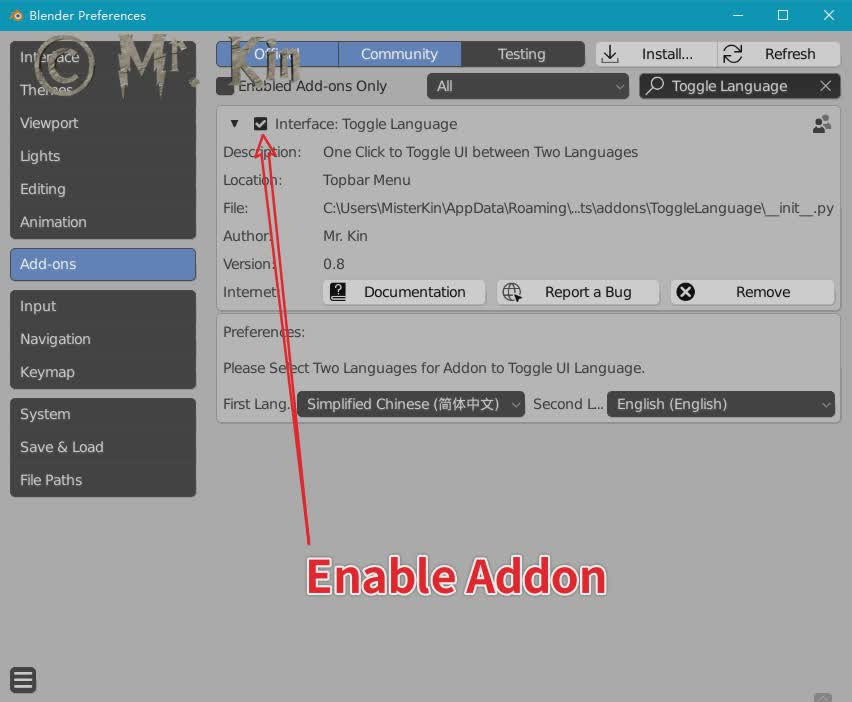
\includegraphics[scale=0.26]{EnableAddon}
        \caption{启用插件}
        \label{启用插件}
    \end{minipage}
\end{figure}

\subsection{插件UI}
\label{插件UI小节}
如图\myref{插件UI}所示,启用插件后,可看见插件位于顶端菜单栏末尾处。插件UI从左往右看,有三个元素:
\begin{enumerate}
    \item 左侧是语言切换按钮。
    \item 中间是插件的个性化设置菜单。
    \item 右侧是用户偏好设置按钮。
\end{enumerate}

\begin{figure}[h!]
    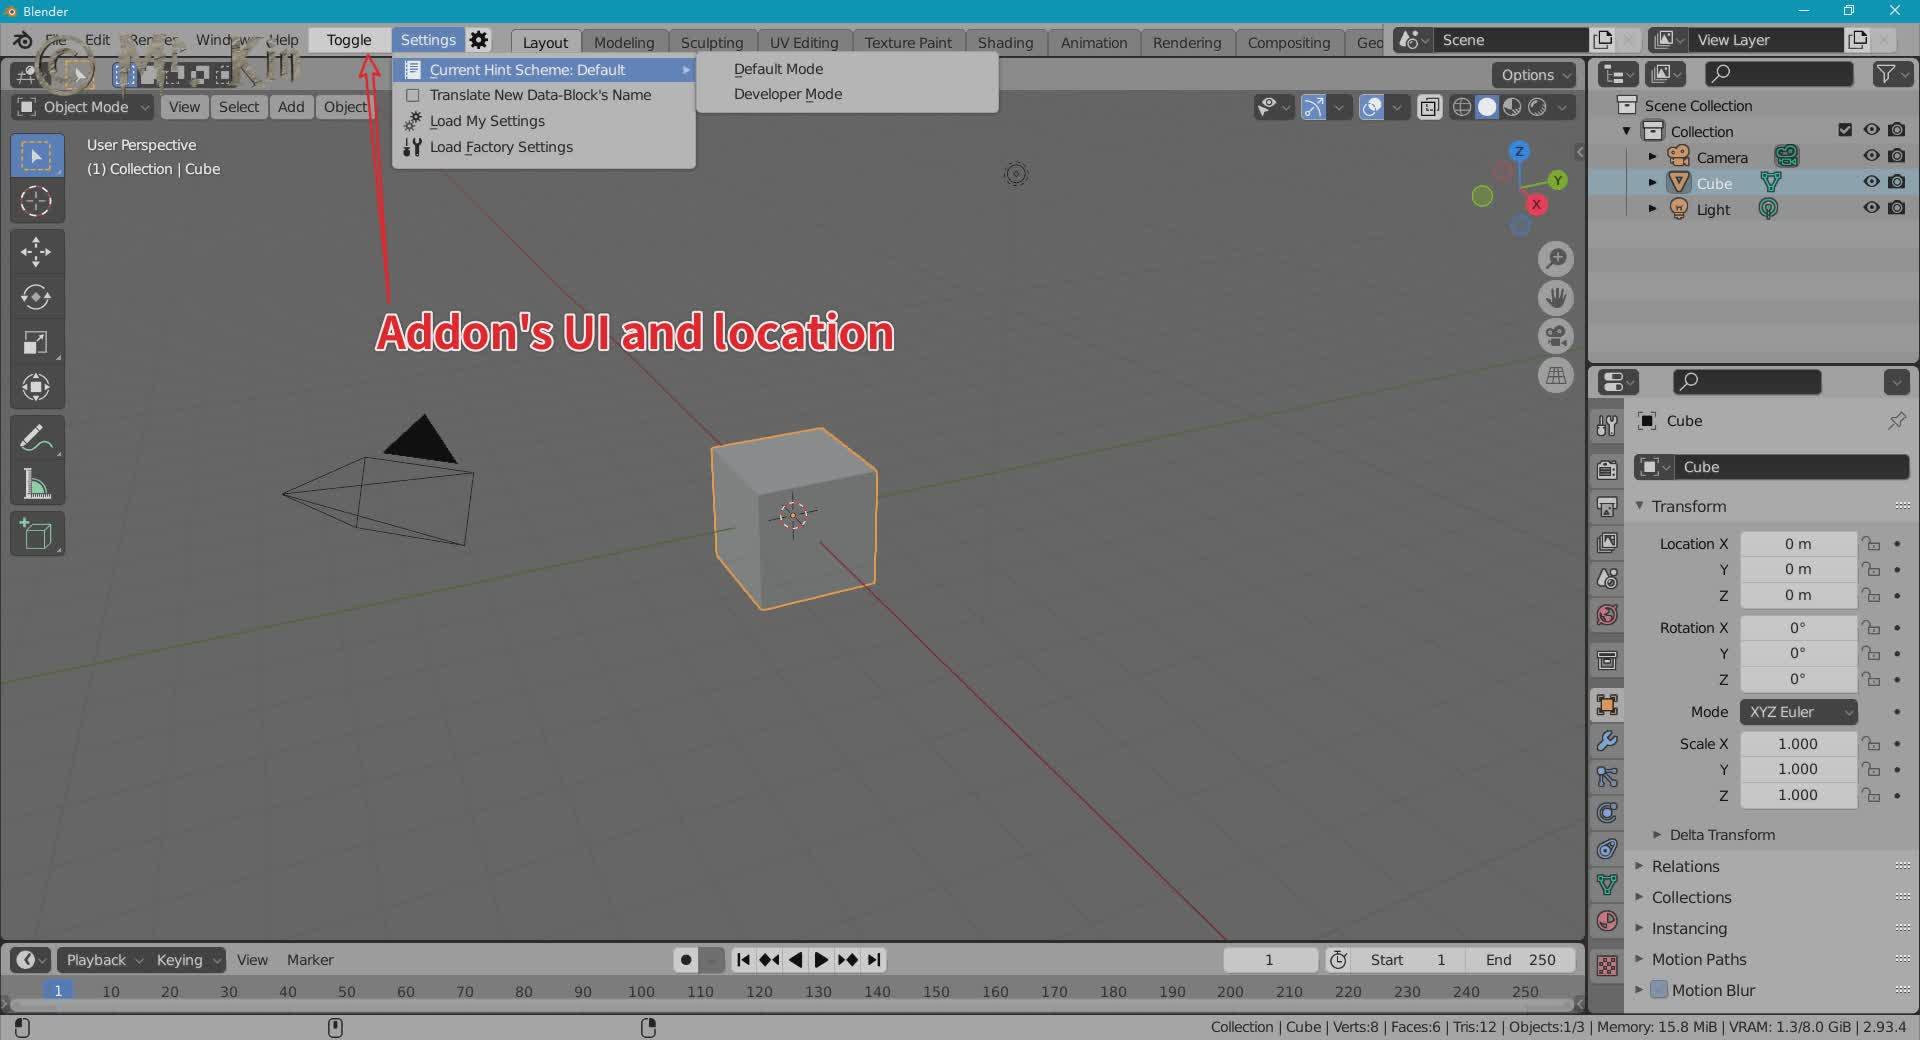
\includegraphics[scale=0.235]{UI}
    \caption{插件UI(图示菜单已被下拉展开)}
    \label{插件UI}
\end{figure}

\subsection{插件功能}
\hypertarget{AddonFeatures}{}

\note{以下按照UI排布位置进行功能介绍。UI排布位置详见「\nameref{插件UI小节}」小节。}

\begin{enumerate}
    \item 语言切换按钮(快捷键F5):切换blender用户界面语言(支持17种语言)。
    \item 设置菜单:插件的个性化设置。
    \begin{enumerate}
        \item UI提示方案菜单:选择相应UI提示的方案。
        \begin{enumerate}
            \item 默认模式:禁用「开发选项」「Python工具提示」,如图\myref{默认提示方案}所示。
            \item 开发者模式:启用「开发选项」「Python工具提示」,如图\myref{开发者提示方案}所示。
        \end{enumerate}
        \item 翻译新建数据块名称按钮:启用/禁用新建数据块名称的翻译功能\footnote{该功能会接管用户偏好设置中的对应功能,这意味着你将无法通过用户偏好设置来修改这个功能。},默认值为禁用,如图\myref{插件的翻译名称选项}所示,其对应在偏好设置中的选项如图\myref{原始的翻译名称选项}所示。在非英语界面环境中,启用该功能可使blender新建数据块的名称为当前语言,如图\myref{翻译名称的效果}所示,新建平面的名称为「平面」,而非「plane」。
        \item 加载我的设置按钮({\color{red}试验性,慎用}):部署我个人的偏好设置。所涉及的设置选项详见\hyperlink{MySettings}{我的设置}。该功能会覆盖你原有的blender设置(启动文件和偏好设置),请详细了解所涉及的设置项后再确认是否使用该功能。目前该功能仅支持拥有英伟达显卡的win平台(默认路径安装),其他系统平台或者其他安装路径的用户使用该功能可能会有报错。\footnote{因为涉及到blender主题文件路径和Cycles引擎渲染设备的选择,暂不支持全平台任意路径安装的情况。}
        \item 加载初始设置按钮:加载初始的偏好设置和启动文件,即重置blender,还原成初次安装时的状态。
    \end{enumerate}
    \item 用户偏好设置按钮(快捷键Ctrl+Alt+U):打开用户偏好设置窗口。
\end{enumerate}

\subsubsection{其他功能}
搜索功能增设\footnote{在blender v2.93.3版本测试中,已经不是增设效果,本插件的F6键会自动替代原F3键。}快捷键F6。(因本人有其他软件占用全局快捷键F3,故增设F6键)

\subsubsection{插件切换语言的设置}
在本插件的偏好设置面板中,可以设置切换语言功能所需的语言项,如图\myref{启用插件}所示,两个语言项的默认值分别为简体中文和英语。两个语言项不分前后顺序,只要设置好两种不同语言,插件便可以在这两种语言之间切换UI界面。目前本插件支持17种语言\footnote{即blender UI翻译语言中Complete和In Progress两个列表中的语言。暂不考虑加入Starting列表中的语言,因为其变动性较高,有可能被删除或者新添加。}相互切换。

\begin{figure}[h!]
    \begin{minipage}[t]{0.47\textwidth}
        \includegraphics[scale=0.26]{DefaultHint}
        \caption{UI提示方案菜单:默认模式}
        \label{默认提示方案}
    \end{minipage}
    \quad
    \begin{minipage}[t]{0.47\textwidth}
        \includegraphics[scale=0.26]{DeveloperHint}
        \caption{UI提示方案菜单:开发者模式}
        \label{开发者提示方案}
    \end{minipage}

    \vspace{1ex}

    \begin{minipage}[t]{0.47\textwidth}
        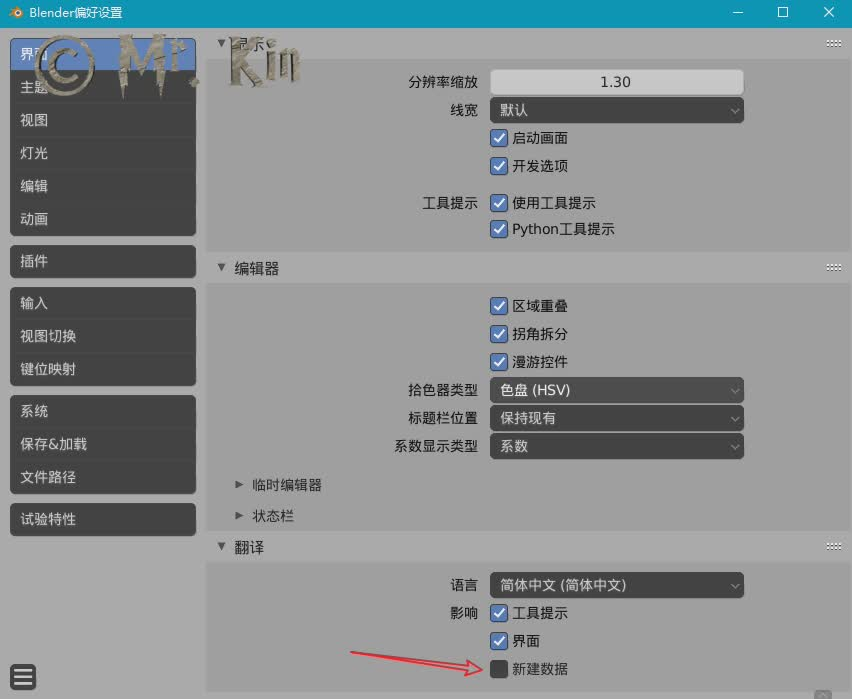
\includegraphics[scale=0.26]{TranslateNameOptionOrigin}
        \caption{原始的翻译新建数据块名称选项}
        \label{原始的翻译名称选项}
    \end{minipage}
    \quad
    \begin{minipage}[t]{0.47\textwidth}
        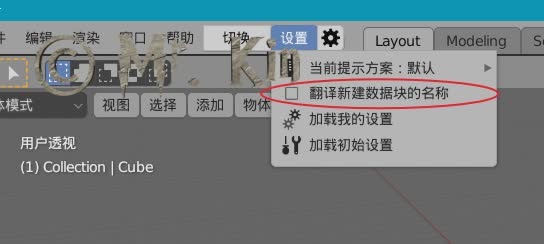
\includegraphics[scale=0.41]{TranslateNameOptionAddon}
        \caption{插件的翻译新建数据块名称选项}
        \label{插件的翻译名称选项}
    \end{minipage}

    \vspace{1ex}

    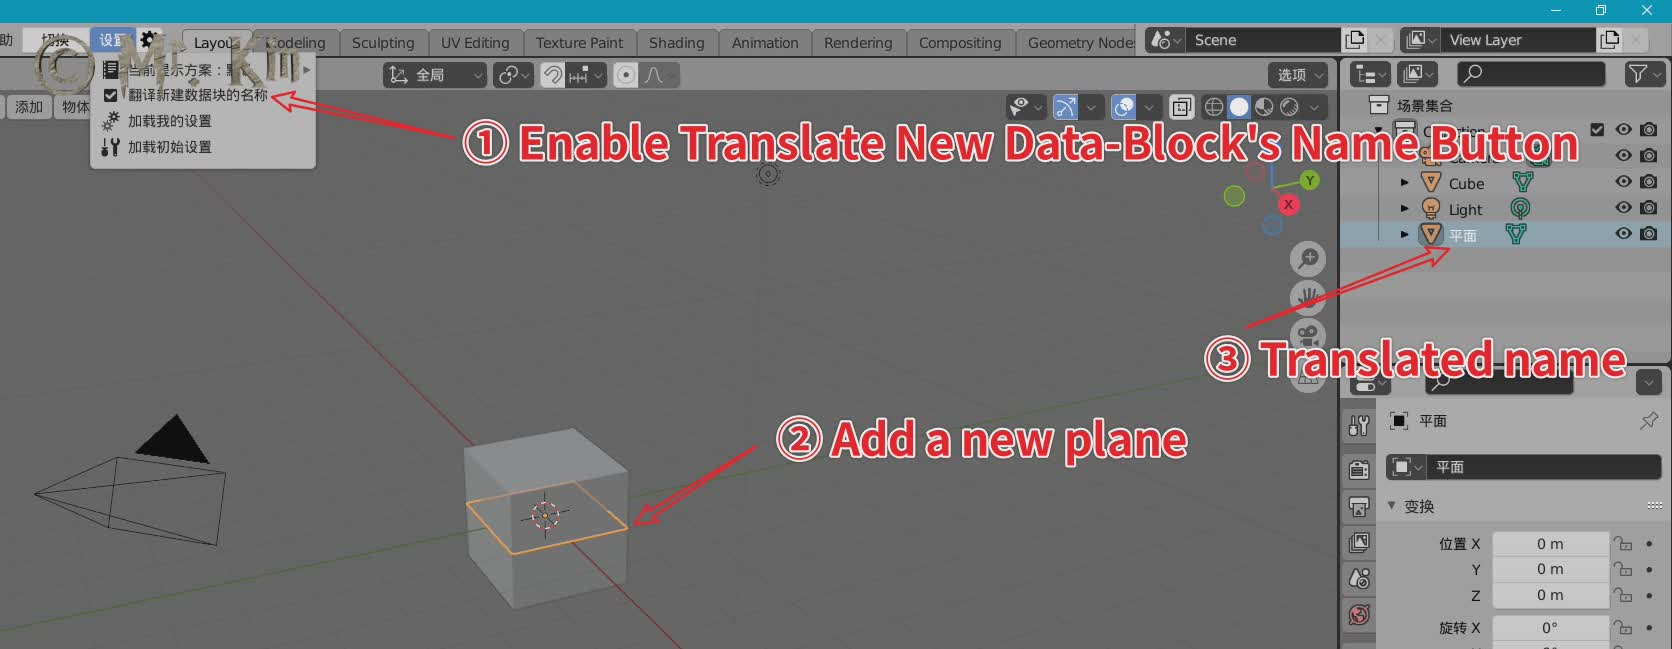
\includegraphics[scale=0.27]{TranslateNameEffect}
    \caption{翻译新建数据块名称的效果(图示界面语言为简中)}
    \label{翻译名称的效果}
\end{figure}

\newpage
\subsubsection{我的设置(我本人的一些blender设置参数)}
\hypertarget{MySettings}{}
\begin{enumerate}
    \item 偏好设置部分:
    \begin{enumerate}
        \item 界面>分辨率缩放到1.3
        \item 主题> Blender Light
        \item 插件>启用插件Node Wrangler、Cell Fracture、Auto Tile Size、Development: Icon Viewer
        \item 视图切换>启用「围绕选择物体选择」和「缩放至鼠标位置」
        \item 键位映射>启用「Pie Menu on Drag」和「Extra Shading Pie Menu Items」
        \item 系统
        \begin{enumerate}
            \item Cycles渲染设备> CUDA
            \item 声音>音频设备> SDL
        \end{enumerate}
        \item 报错\&加载>启用「压缩文件」、关闭「自动保存」
        \item 文件路径
        \begin{enumerate}
            \item 纹理:H:\textbackslash Textures\textbackslash
            \item 临时文件:E:\textbackslash Temp\textbackslash
            \item 渲染输出:E:\textbackslash Process\textbackslash
            \item 渲染缓存:E:\textbackslash Temp\textbackslash
        \end{enumerate}
    \end{enumerate}
    \item 启动文件部分(注意:使用「我的设置」功能,会同时将以下设置保存进启动文件):
    \begin{enumerate}
        \item 属性编辑器
        \begin{enumerate}
            \item 渲染属性
            \begin{enumerate}
                \item 渲染引擎> Cycles
                \item 设备> GPU计算
                \item 采样>启用「自适应采样」
                \item 性能> Auto Tile Size > Target Tile Size > 256
                \item 性能>线程>多线程模式>固定
                \item 性能>线程>线程> 6
            \end{enumerate}
            \item 输出属性>输出路径:E:\textbackslash Process\textbackslash
        \end{enumerate}
    \end{enumerate}
    \item 状态栏>启用「场景统计数据」「系统内存」「显存」
\end{enumerate}

\section{开发记录}
\subsection{已知问题}
\subsubsection{翻译新建数据块名称按钮设置值无法随用户偏好设置保存}
该功能的代码实现:其property属性值是注册在bpy.types.Scene中。因此,无法通过用户偏好设置中自动保存设置的功能进行存储。不像本插件偏好设置面板中的两种语言的属性值,后者是通过bpy.types.AddonPreferences类实现的,它可以通过用户偏好设置中自动保存设置的功能进行存储\footnote{实际上,在禁用用户偏好设置的自动保存设置功能后,本插件偏好设置面板中的两种语言的属性值也无法自动存储,需要保存在某一工程文件中才行。}。

建议:若需要保存该功能的设置值,请保存一个工程文件\footnote{保存在启动文件也是可行的。}(.blend),该功能的设置值会保存在这个工程文件。

\subsubsection{加载初始设置按钮会有机率导致blender闪退}
在未保存工程文件\footnote{指通过安装路径打开主程序的情况或者打开一个工程文件后进行修改却未保存的情况。}(.blend)的情况下,加载初始设置功能会有机率引起异常码EXCEPTION\_ACCESS\_VIOLATION,从而导致blender闪退,目前暂未查明原因。在导致blender闪退时,重置功能的代码执行的不完整,一般是成功地加载初始偏好设置并保存,而初始启动文件并未成功加载并保存。因此,在该功能导致blender闪退后,还请用户自行重置偏好设置及启动文件。

建议:在使用该功能之前,请先保存一个工程文件(.blend)。

\subsection{开发环境}
\begin{itemize}
    \item OS: Win10 v21H1
    \item Blender: v2.93.4
\end{itemize}

\newpage
\subsection{更新历史}
表\myref{更新历史}记录了本插件的各个版本更新历史。
\begin{table}[h!]
    \caption{插件的更新历史}
    \label{更新历史}
    \begin{tabular}{|*{2}{c|}m{305pt}|}
        \hline
        版本 & 更新日期 & \multicolumn{1}{c|}{更新内容} \\
        \hline
        v0.8 & 2021/8/30 & 支持切换更多语言;支持完整翻译插件UI;为某些功能添加交互提示(信息框,确认框等)…… \\
        \hline
        v0.7 & 2021/7/11 & 我的偏好设置支持blender v2.93;重写property代码 \\
        \hline
        v0.6 & 2021/3/10 & 添加布尔值按钮-新数据翻译;支持快捷键;代码重构,插件翻译重构…… \\
        \hline
        v0.5 & 2020/12/8 & 支持blender v2.91;支持从.zip文件安装插件…… \\
        \hline
        v0.5-beta & 2020/9/20 & 添加菜单用以选择UI提示方案 \\
        \hline
        v0.4 & 2020/8/3 & 代码项目重命名为ToggleLanguage;按钮UI放置于最右端;添加新按钮以快速查看preferences \\
        \hline
        v0.3 & 2020/6/5 & 更新至blender 2.83 API;修改部分类名;添加文档链接;修改完善许可说明 \\
        \hline
        v0.2 & 2020/5/21 & 清除未使用属性的报错 \\
        \hline
        v0.1 & 2020/5/12 & 完成基础的功能设计「一键切换」 \\
        \hline
    \end{tabular}
\end{table}

\note{更多详细的信息,请查看 \href{https://github.com/Mister-Kin/ToggleLanguage/releases}{Release Notes}。}

\section{作者}
\textbf{ToggleLanguage} © Mr. Kin, 项目代码采用 \href{https://github.com/Mister-Kin/ToggleLanguage/blob/master/LICENSE}{GNU GPL v3.0} 许可协议进行发布。

由 Mr. Kin 著作并维护。

\inputBibliography
\appendix
% 附录

\end{document}
